\section{Multilagen-PVD}
\label{multilayer}

\todo{Auf GMR/TMR-Systeme eingehen}
\todo{Auf Röntgen-Optiken eingehen}
\todo{Korrelierte Rauheit?}
Mit PVD-Methoden können auch mehrlagige Schichten abgeschieden werden, die im folgenden Kapitel am Beispiel von dünnen Cu/Ni-Multilagen näher untersucht werden sollen.
Das Kupfer-Nickel-System wurde aufgrund ähnlicher Gitterkonstanten gewählt (Ni:~\SI{3.52}{\angstrom}, Cu:~\SI{3.61}{\angstrom}), die kristallines Wachstum ermöglichen und somit Fehlstellen unterbinden.
Durch die Ähnlichkeit zur Kupfer-PVD lässt sich der Prozess zudem auf den dort entwickelten Prozessparametern und den untersuchten Potentialparametersätzen aufbauen.

Im Experiment werden mehrlagige Kupfer-Nickel-Schichten per Elektro\-deposition\cite{yang_pulsed_1995} oder durch Sputtern\cite{cammarata_nanoindentation_1990} hergestellt, wobei üblicherweise Lagendicken im Bereich mehrerer Nanometer erzielt werden.
Dieses Vorgehen lässt sich direkt in Parsivald-Simulationen übertragen, in denen zugunsten der Rechenzeit in den folgenden Untersuchungen vergleichsweise dünne Lagen mit einer Dicke von \SI{1}{\nano\meter} abgeschieden wurden.
Anschließend werden diese auf Ähnlichkeit mit LAMMPS-präparierten Multilagen hinsichtlich ihrer Lagendicke und -rauheit untersucht.
Eine Auswertung der relativen Verteilung der Spezies entlang der Abscheidungsrichtung wird ergänzend für verschiedene Relaxationszeiten als Maß der Lagenqualität durchgeführt.
Abscheidungen von Lagen mit einer Dicke von \SI{6}{\nano\meter} wurden ebenfalls mit Parsivald simuliert, doch mangels verfügbarer Rechenzeit für vergleichbare LAMMPS-Simulationen nicht eingehender untersucht.

Wie bei den Gold-PVD-Simulation zuvor müssen für erfolgreiche Simulationen einige Prozessparameter wie Relaxationszeit, Thermostatdämpfung und Substrattemperatur optimiert werden.
Als Zielgrößen für die Optimierung wurden zur Vermeidung von Fehlstellen die Rauheit der Oberfläche und die Qualität der einzelnen Lagen im Vergleich mit ähnlichen Untersuchungen\cite{zhou_atomistic_1998} gewählt.
In diesen Untersuchungen wurde bereits gezeigt, dass die kinetische Energie der einfallenden Atome einen erheblichen Einfluss auf die Qualität der einzelnen Lagen hat, weshalb gleichartige Untersuchungen nur hinsichtlich der Substrattemperatur durchgeführt wurden.

\subsection{Ergebnisse}

Parsivald-Simulationen erzeugen nach korrekter Parametereinstellung monokristallin gewachsene, klar abgegrenzte Atomlagen geringer Rauheit, die sich gut mit den Ergebnissen gleichartiger LAMMPS-Simulationen decken (Abbildung~\ref{fig:multilayerresults}).
RMS-Rauheiten um \SI{1.2}{\angstrom} stellen sich mit beiden Simulationsmethoden bis zur zehnten Lage ein und stimmen somit miteinander und mit den bisherigen Ergebnissen überein (Abbildung~\ref{fig:multilayerplots-a}).

Zuvor war eine Anpassung der Temperaturen und Relaxationszeiten notwendig, die jedoch für LAMMPS und Parsivald gleichermaßen gelten.
Als Richtwert wurde die Qualität der einzelnen Lagen in Form des Anteils der Spezies in Abhängigkeit der Höhe über dem Substrat genutzt (Abbildung~\ref{fig:multilayerplots-b}).
Lagen schlechterer Qualität zeigen eine höhere Durchmischung der Schichten, was wiederum zu einer Senkung der relativen Häufigkeit einer Spezies innerhalb ihrer Schicht führt, wie für die beiden Verteilungen bei einer Relaxationszeit von \SI{0.2}{\femto\second} pro Ereignis beobachtet werden kann.
Erst bei Verdopplung der Relaxationszeit bilden sich klar abgegrenzte Lagen aus, wie sie in Abbildung~\ref{fig:multilayerresults} dargestellt sind.

In Anhang~\ref{appendix:multilayer} ist eine Auswahl von mehrlagigen Kupfer-Nickel-Schichten dargestellt, die durch Unterrelaxation verursachte strukturelle Fehler aufweisen.
Bei größeren Systemen ist zudem mit Verspannungen aufgrund der unterschiedlichen Bindungslängen Gitterversetzungen und Fehlstellen zu rechnen, die allerdings durch Finite-Size-Effekte unterdrückt sein können.

\begin{figure}
  \captionsetup[subfigure]{singlelinecheck=false}
  \def\subfigwidth{7cm}
  \begin{subfigure}[t]{\subfigwidth}
    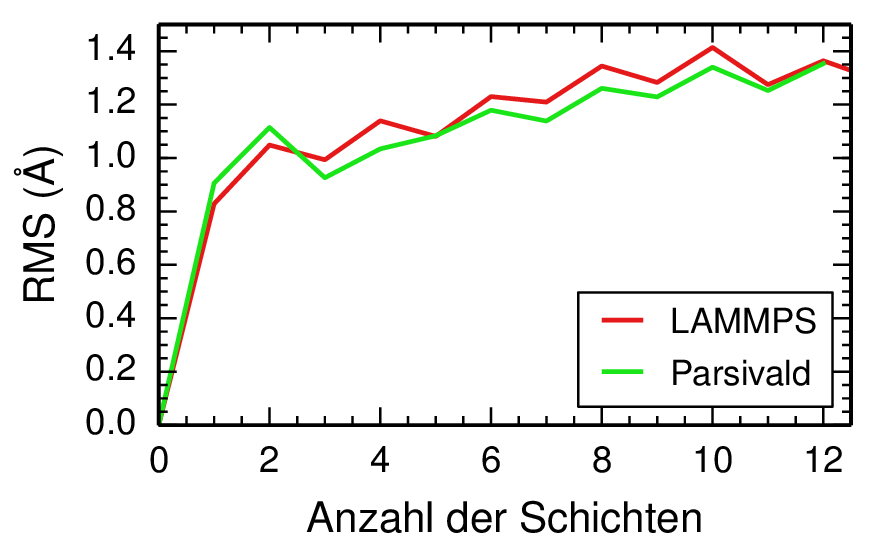
\includegraphics[width=\textwidth]{CuNi_layerroughness_comparison}
    \subcaption{
      Vergleich der Lagen-Rauheit (Abb.~\ref{fig:multilayerresults})
    }
    \label{fig:multilayerplots-a}
  \end{subfigure}
  \hfill
  \begin{subfigure}[t]{\subfigwidth}
    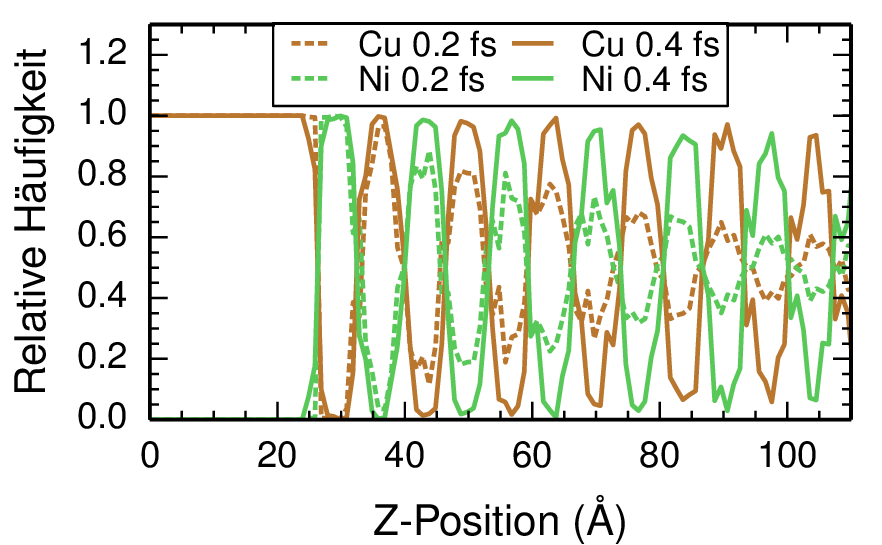
\includegraphics[width=\textwidth]{CuNi_atomdistribution_relax}
    \subcaption{Einfluss von $t_\text{relax}$ auf die Lagen-Qualität}
    \label{fig:multilayerplots-b}
  \end{subfigure}
  \caption[Rauheit und Qualität von Kupfer-Nickel-Multilagen]{
    Rauheit und Qualität von Kupfer-Nickel-Multilagen
  }
  \label{fig:multilayerplots}
\end{figure}

\begin{figure}
  \captionsetup[subfigure]{singlelinecheck=false}
  \def\subfigwidth{7cm}
  \begin{subfigure}[t]{\subfigwidth}
    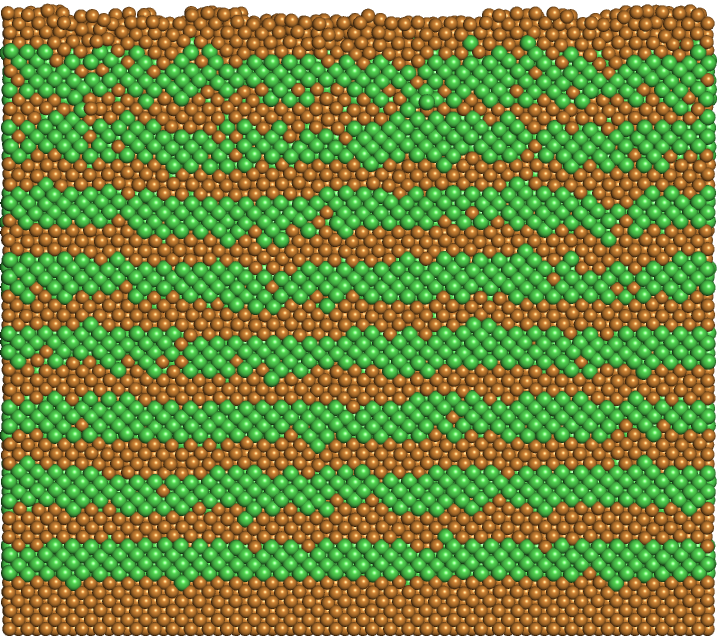
\includegraphics[width=\textwidth]{CuNi_profile_LAMMPS_nice}
    \subcaption{Profil von \ce{CuNi}-Multilagen mit LAMMPS}
  \end{subfigure}
  \hfill
  \begin{subfigure}[t]{\subfigwidth}
    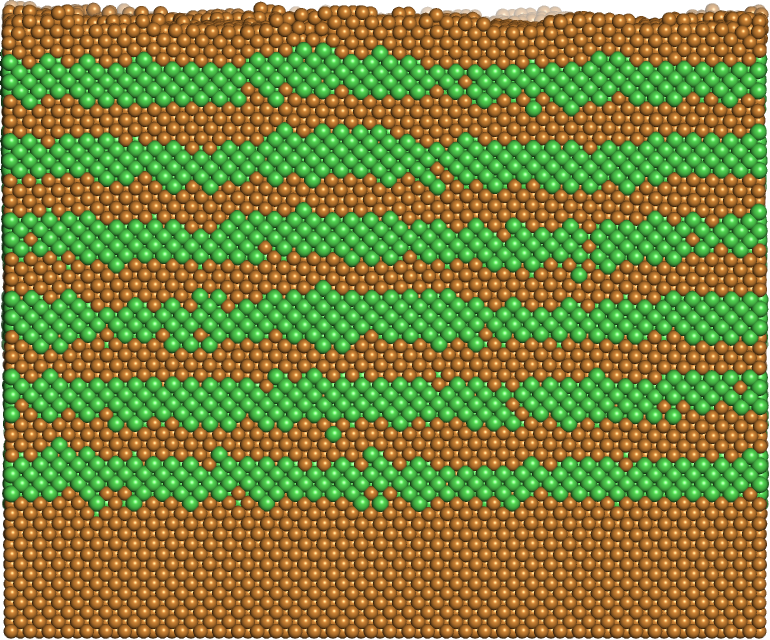
\includegraphics[width=\textwidth]{CuNi_profile_Parsivald}
    \subcaption{Profil von \ce{CuNi}-Multilagen mit Parsivald}
  \end{subfigure}
  \caption{Vergleich von Multilagen-Profilen mit LAMMPS und Parsivald}
  \label{fig:multilayerresults}
\end{figure}
